\section{Exercice 1}
L'objectif de cet exercice est de créer un client et un serveur communiquant à l'aide de sockets non connectées (\emph{DGRAM\_SOCKETS}). Un des points notables de telles sockets est que si des données sont envoyées, elles n'arrivent pas forcément, et si elles arrivent, elles n'arrivent par forcément dans l'ordre. Elles sont utiles pour avoir une taille de header plus faible (par rapport à des sockets connectées utilisant TCP) et lorsque la perte de quelques paquets n'a pas d'importance.\\

Le client se connecte au serveur, envoie son PID ainsi que le message passé en argument du programme au serveur, puis le serveur envoie au client son PID ainsi que le message précédemment reçu.

\subsection{Client}
Du côté du client, nous souhaitons tout d'abord récupérer l'adresse du serveur à l'aide de son nom (e.g. localhost $\rightarrow$ 127.0.0.1) grâce à la fonction \emph{gethostbyname()}. Une fois cela fait, nous créons la datagram socket.\\

\begin{mdframed}[backgroundcolor=hintbg, linecolor=hintborder]
La fonction \emph{gethostbyname()} est dépréciée, la page de manuel de la fonction conseille d'utiliser \emph{getaddrinfo()} à la place. \emph{gethostbyname()} sera principalement utilisée dans ce TP, ayant commencé à travailler avec. Nous aurons cependant l'occasion de voir l'utilisation de \emph{getaddrinfo()} dans l'exercice 2, deux versions du client ayant été développées.
\end{mdframed}

\begin{mdframed}[backgroundcolor=lightblue2, linecolor=darkblue]
Il est à noter que le pointeur vers la structure \emph{hostent} renvoyé par la fonction \emph{gethostbyname()} ne doit pas être libéré. Celui-ci peut pointer vers des données statiques.

%\begin{mdframed}[backgroundcolor=hintbg, linecolor=hintborder]
\begin{mdframed}[backgroundcolor=lightblue, linecolor=darkblue]
	\textbf{gethostbyname(3) man page} :\\ % TODO http://man7.org/linux/man-pages/man3/gethostbyname.3.html
	``The functions gethostbyname() and gethostbyaddr() may  return  pointers to  static  data, which may be overwritten by later calls.''
\end{mdframed}
\begin{mdframed}[backgroundcolor=lightblue, linecolor=darkblue]
	\noindent\textbf{MSDN hostent structure} :\\ % TODO http://msdn.microsoft.com/en-us/library/windows/desktop/ms738552%28v=vs.85%29.aspx
	``An application should never attempt to modify this structure or to free any of its components.''
\end{mdframed}
\end{mdframed}
\

Nous souhaitons pouvoir envoyer un message au serveur à l'aide de la socket précédemment créée. Pour cela, nous devons utiliser la fonction \emph{sendto} prenant entre autres en paramètre un pointeur vers une structure \emph{sockaddr}. Pour être plus spécifique, nous allons remplir les champs d'une structure \emph{sockaddr\_in} qui est spécifique au protocole IPv4. Cette dernière va permettre d'indiquer à qui envoyer le message. Toutes les informations pour remplir cette structure sont disponibles: la famille d'adresses (ici \emph{AF\_INET} pour IPv4), le port du serveur (récupéré en argument du programme), et l'adresse du serveur (récupérée à l'aide de \emph{gethostbyname()}).

\begin{lstlisting}
struct sockaddr_in dest_addr;

...

dest_addr.sin_family = AF_INET;
dest_addr.sin_port = htons(atoi(argv[2]));
dest_addr.sin_addr = *((struct in_addr*) he->h_addr_list[0]);
memset(dest_addr.sin_zero, 0, sizeof(dest_addr.sin_zero));
\end{lstlisting}
\

La fonction \emph{sendto()} ne garantie pas que le message soit complétement envoyé, la fonction \emph{sendto\_complete} a donc été créée dans le fichier \emph{socket\_tools.c}. Cette fonction fait appel à \emph{sendto()} tant que la taille des données envoyées est inférieure à la taille totale du message à envoyer.

\begin{lstlisting}
int sendto_complete(int sockfd, char* msg, int msg_size,
    const struct sockaddr *dest_addr)
{
    int sent_size = 0;

    while (sent_size < msg_size) {
        int remaining_size = msg_size - sent_size;
        int temp_size = sendto(sockfd, msg + sent_size, remaining_size, 0,
        dest_addr, sizeof(*dest_addr));
        if (temp_size == -1) {
            perror("sendto");
            break;
        }

        sent_size += temp_size;
    }

    return (sent_size != msg_size) ? -1 : 0;
}
\end{lstlisting}
\

Une fois le message complétement envoyé, on souhaite recevoir la réponse du serveur. Pour cela on utilise la fonction \emph{recvfrom\_helper()} définie dans \emph{socket\_tools.c}. Celle-ci exécute l'appel système \emph{recvfrom()} permettant de recevoir des données via des \emph{SOCK\_DGRAM}, puis s'assure que le message se termine par le caractère \textbackslash 0.

\begin{lstlisting}
int recvfrom_helper(int sockfd, char *buffer, int buffer_size, int *recv_size,
    struct sockaddr *src_addr, socklen_t *addrlen)
{
    *recv_size = recvfrom(sockfd, buffer, buffer_size, 0, src_addr, addrlen);
    if (*recv_size == -1) {
        perror("recvfrom");
        return -1;
    }

    // Make sure the received message ends with '\0'.
    if (buffer[*recv_size - 1] != '\0') {
        if (*recv_size == buffer_size) {
            buffer[*recv_size - 1] = '\0';
        }
        else {
            buffer[*recv_size] = '\0';
        }
    }

    return 0;
}
\end{lstlisting}

\subsection{Serveur}
Pour le serveur, la socket est tout d'abord créée puis liée à toute les interfaces et à un port spécifique. La création se fait comme précédemment à l'aide de l'appel système \emph{socket()}, et la liaison se fait à l'aide de \emph{bind()} et d'une structure \emph{sockaddr\_in}. Le port passé en argument du programme est utilisé pour le champ \emph{sin\_port} de la structure, et INADDR\_ANY est passé au champ \emph{sin\_addr.s\_addr}. Cette constante indique que la socket est liée à toutes les interfaces locales. \cite{cite:cmu_edu_inaddr_any} \cite{cite:man_ip}

\begin{mdframed}[backgroundcolor=lightblue, linecolor=darkblue]
\textbf{ip(7) man page :}\\
``When INADDR\_ANY is specified in the bind call, the  socket will be bound to all local interfaces.''
\end{mdframed}

\begin{mdframed}[backgroundcolor=hintbg, linecolor=hintborder]
INADDR\_ANY est représenté par l'adresse \emph{0.0.0.0}, et vaut donc \emph{0x000000} en représentation hexadécimale. Passer cette constante à la fonction \emph{htonl()} n'est donc pas utile, puisque sa valeur hexadécimale est la même en big-endian et en little-endian.
\end{mdframed}
\newpage

\begin{lstlisting}
// Create socket (IPv4, connectionless, UDP)
sockfd = socket(AF_INET, SOCK_DGRAM, 0);
if (sockfd == -1) {
    perror("server - socket init");
    return EXIT_FAILURE;
}

// fill serv_addr
serv_addr.sin_family = AF_INET;
serv_addr.sin_port = htons(atoi(argv[1]));
serv_addr.sin_addr.s_addr = INADDR_ANY;
memset(serv_addr.sin_zero, 0, sizeof(serv_addr.sin_zero));

// bind socket to all local interfaces on the port specified in argument
status = bind(sockfd, (struct sockaddr *) &serv_addr, sizeof(serv_addr));
if (status == -1) {
    perror("server - bind");
    return EXIT_FAILURE;
}
\end{lstlisting}
\

Une fois la socket initialisée, le principe est similaire à celui du client. Des données sont tout d'abord reçues d'un client à l'aide de \emph{recvfrom\_helper}, puis le message est traité afin de remplacer le PID du client par celui du serveur, et enfin le message ainsi modifié est envoyé au client à l'aide de \emph{sendto\_complete}. Ces étapes sont effectuées dans une boucle afin de pouvoir traiter les messages de plusieurs clients.

\subsection{Exemple d'exécution}
\begin{figure}[h!]
	\centering
	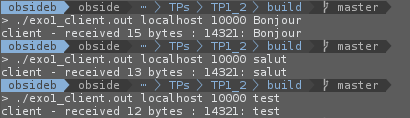
\includegraphics[width=0.8\textwidth]{screenshots/ex1_client.png}
	\caption{exo1\_client.out}
\end{figure}

\begin{figure}[h!]
	\centering
	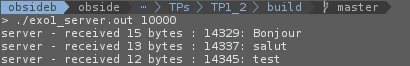
\includegraphics[width=0.8\textwidth]{screenshots/ex1_server.png}
	\caption{exo1\_server.out}
\end{figure}
